%-------------------------------------------------------------------------------
% seq66 setmaster
%-------------------------------------------------------------------------------
%
% \file        seq66 setmaster.tex
% \library     Documents
% \author      Chris Ahlstrom
% \date        2020-01-13
% \update      2020-01-13
% \version     $Revision$
% \license     $XPC_GPL_LICENSE$
%
%     Provides a discussion of the MIDI GUI setmaster that Seq66
%     supports.
%
%-------------------------------------------------------------------------------

\section{Seq66 Set Master}
\label{sec:setmaster}

   The \textbf{Set Master} is a way to get a global view of all the sets in a
   \textsl{Seq66} MIDI file, and to be able to do some simple operations
   (movement, naming, etc.) with the sets.

   CURRENTLY, this section is a PLACEHOLDER.

\begin{figure}[H]
   \centering 
   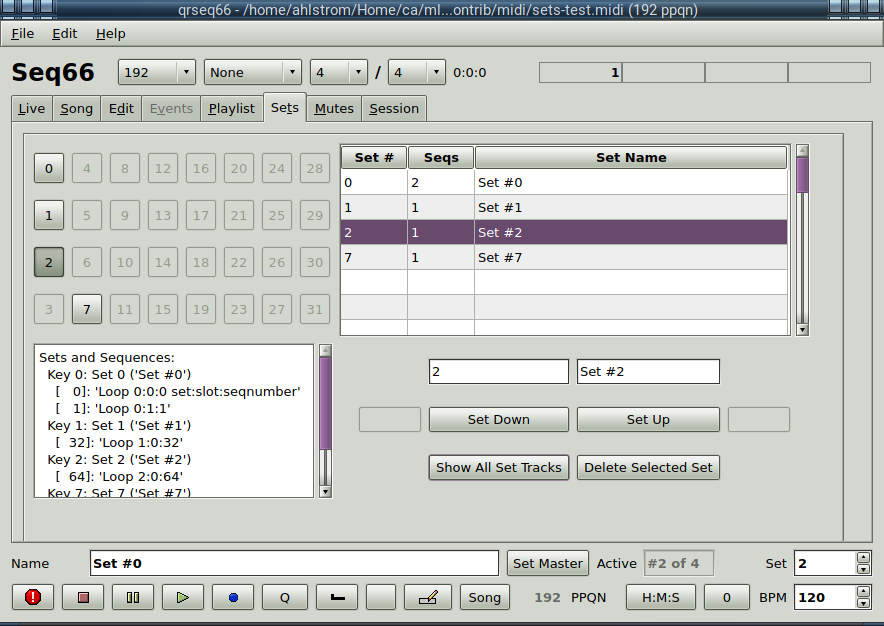
\includegraphics[scale=0.85]{tabs/sets/setmaster-tab.png}
   \caption{Sets Tab}
   \label{fig:setmaster_tab}
\end{figure}

%-------------------------------------------------------------------------------
% vim: ts=3 sw=3 et ft=tex
%-------------------------------------------------------------------------------
